\chapter{Related Work}\label{ch:related-work}

To answer the main thesis question, a review of existing studies will be needed.
The topic of DQ and the cost on business is well researched.
One of the oldest articles was written by Gerald A. Feltham in 1968 with title \enquote{The Value of Information}.
Many articles and studies were written on the topic since then, therefore we can recognize some basic structures when talking about DQ methodology.

\section{Hybrid Approach}

In the article \textit{Data quality assessment: The Hybrid Approach} the authors defined data quality as \enquote{fit for use}.
They reviewed several assessment techniques, including:
\begin{itemize}
    \item AIMQ (Lee et al., 2002),
    \item TQDM (English, 1999),
    \item cost-effect of low data quality (Loshin, 2004) and
    \item subjective-objective data quality assessment (McGilvray, 2008).
\end{itemize}

The result of the study is a general framework for creating customized, bussiness unique data quality assessment process.
The process consists of seven consecutive activities:
\begin{enumerate*}[label=(\roman*)]
    \item select data items,
    \item select a place where data is to be measured,
    \item identify reference data,
    \item identify DQ dimensions,
    \item identify DQ metrics,
    \item perform measurement and
    \item conduct analysis of the results.
\end{enumerate*}

The methodology can be summarized as follows.
The input data (i) are measured (vi) and thus the dimensions (iv) and metrics (v) are obtained.
Metrics are applied to the data in the central repository (ii).
If necessary, the data may be validated against the reference data (iii).

\begin{figure}[htb]
    \centering
    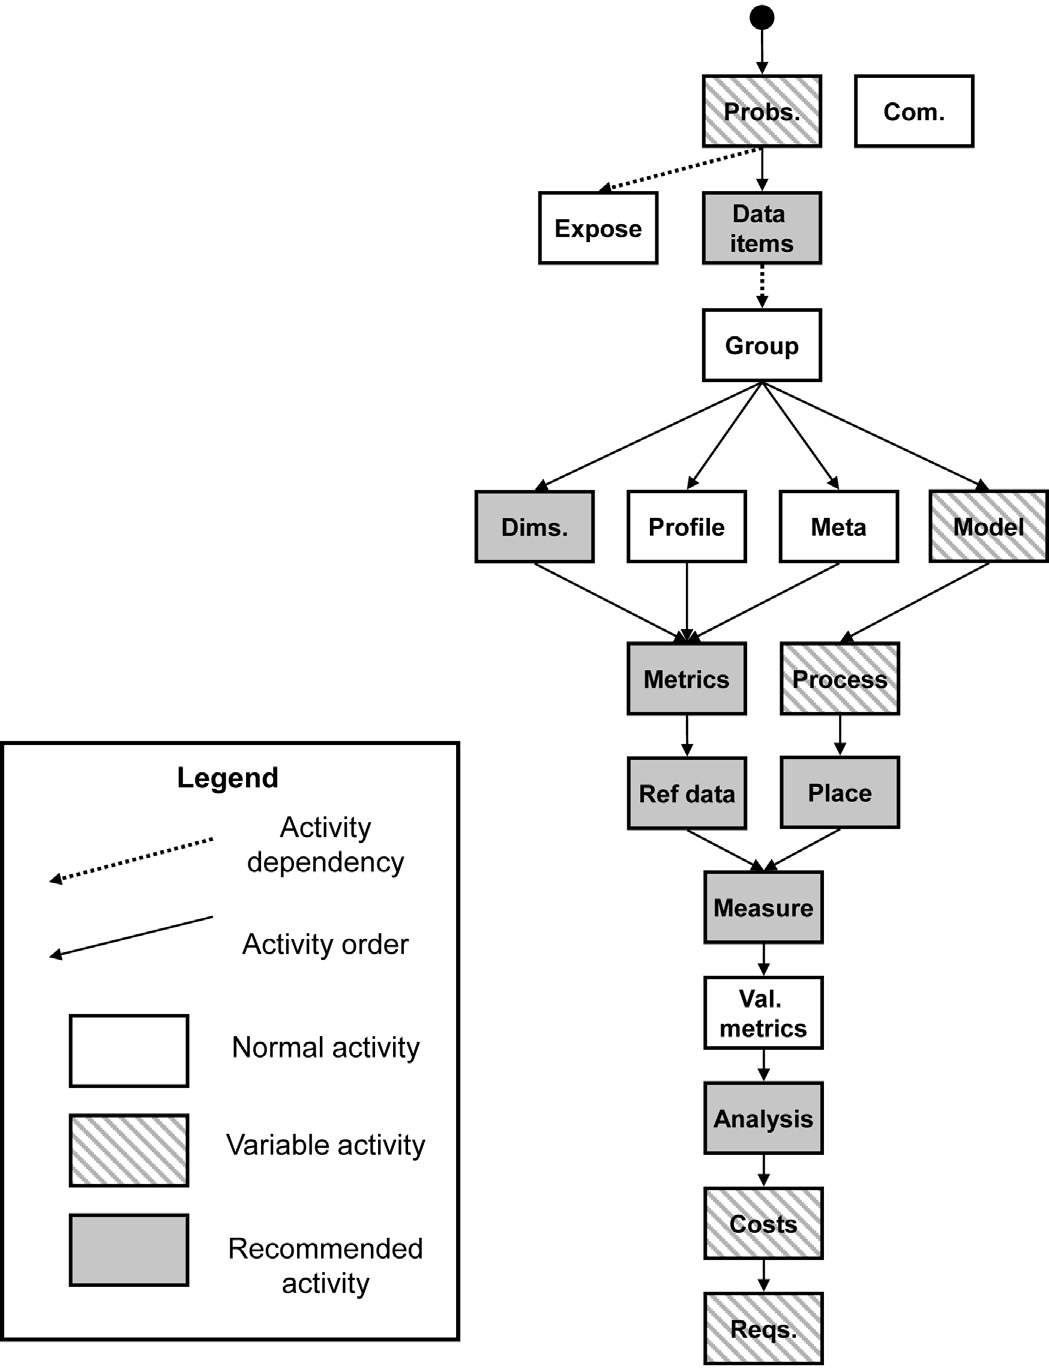
\includegraphics[width=0.4\textwidth]{figures/hybrid-generic-at.jpg}
    \caption{A generic AT according to the Hybrid Approach methodology~\cite{woodal2013}}
    \label{fig:hybrid-generic-at}
\end{figure}
\FloatBarrier

The methodology is tested by the authors on two practical cases.
The first use case is to adapt the framework for an MRO (Maintenance Repair and Operations) company.
The second use case is the adaptation of the methodology for the London Underground.

A very important result of the study is a configurable process model.
It is possible to design an alternative configuration of the process model to suit the case study or specific domain.

\begin{figure}[htb]
    \centering
    
    \begin{subfigure}{0.45\textwidth}
        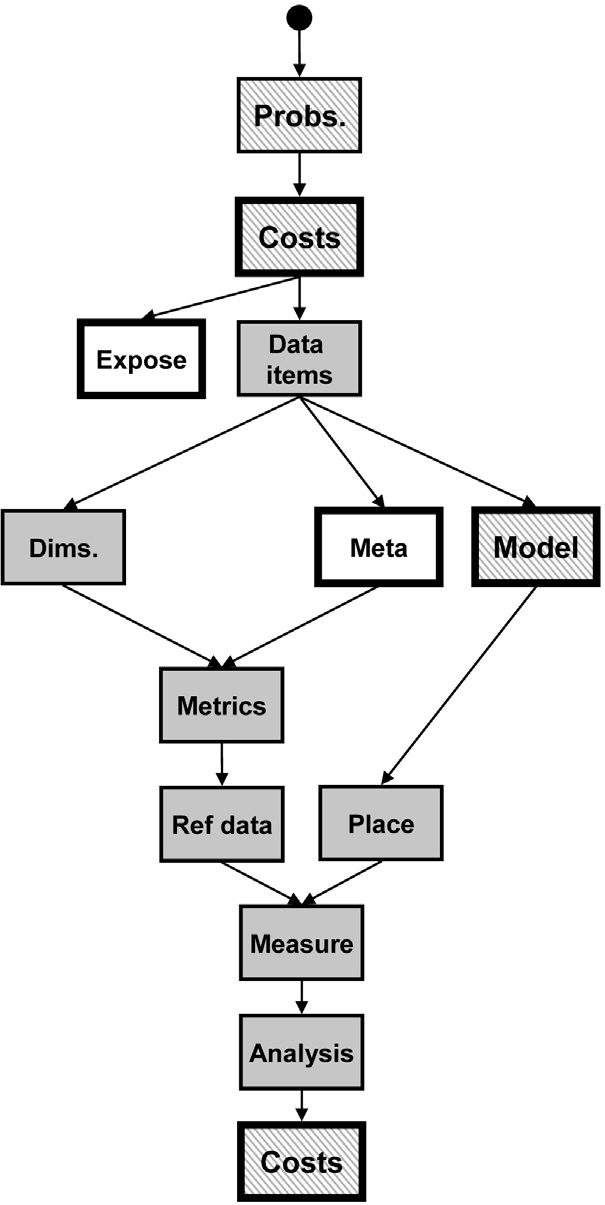
\includegraphics[height=6cm]{figures/hybrid-at-mro.jpg}
        \centering
        \caption{An AT for the MRO organisation}
        \label{fig:subim1}
    \end{subfigure}
    \begin{subfigure}{0.45\textwidth}
        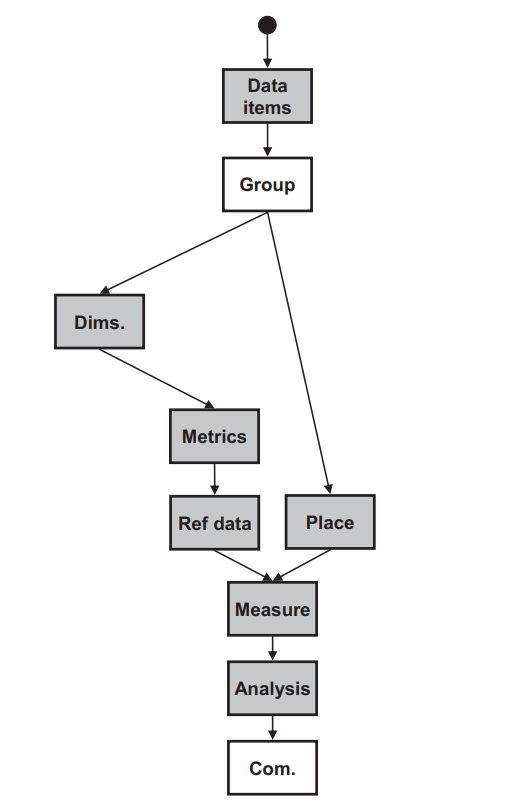
\includegraphics[height=6cm]{figures/hybrid-at-lu.png}
        \centering
        \caption{An AT for London Underground}
        \label{fig:subim2}
    \end{subfigure}

    \caption{ATs for the case studies~\cite{woodal2013}}
    \label{fig:image2}
\end{figure}
\FloatBarrier

In the \textit{Hybrid Approach}, the ATs developed between 1998 and 2008 were incorporated, and they all suggest very similar ideas to evaluating DQ~\cite{woodal2013}.
The methodology, thanks to the fact that it takes over the best practices of other methodologies, will be up-to-date for a long time.
The only problem arises when multiple stakeholders demand conflicting requirements.
If one party requires some activity and the other does not, the activity cannot simply be incorporated due to time and resource costs.
A thorough analysis is needed in this regard.

\section{AIM Quality}

The AIM Quality is a information quality assessment and benchmarking methodology for Management Information Systems (MIS).
The methodology consists of three main components, a model, a questionnaire to measure information quality, and analysis techniques for information quality interpretation.
The methodology has been built on the foundations of other academic studies (e.g., Wang \& Strong, Goodhue, Jarke \& Vassiliou) as well as professional white-papers (e.g., Department of Defense, HSBC, and AT\&T), and has been validated on health organizations use cases.

The important components in AIMQ are the IQ dimensions, critical for the information consumers.
The authors grouped IQ dimensions into four categories, \textit{intrinsic} IQ (the information itself contains a certain level of quality), \textit{contextual} IQ (quality must be considered within the business context), \textit{representational} IQ (expressing whether the information is comprehensible in the information system) and \textit{accessibility} IQ (expressing whether the information is accessible in the information system, but at the same time securely stored).

The information quality model in AIMQ, Product Service Provider (PSP/IQ) model, has four quadrants relevant to the IQ improvement decision process.
The model is shown in the Table~\ref{table:psp-iq}.
This model can be used to evaluate how well a company develops \textit{sound} and \textit{useful} information products and delivers \textit{dependable} and \textit{usable} information services to the consumers.

\begin{table}[htbp]
    \centering

    \begin{tabular}{@{}l|ll@{}}
        \toprule
                        & \shortstack{Conforms to \\ specifications}    & \shortstack{Meets or exceeds consumer \\ expectations}    \\ \midrule
        Product Quality & Sound information                             & Useful information                                        \\
        Service Quality & Dependable information                        & Usable information                                        \\
        \bottomrule
    \end{tabular}

    \caption{The PSP/IQ model~\cite{lee2002}}
    \label{table:psp-iq}
\end{table}
\FloatBarrier

\subsection{Four PSP/IQ model quadrants}

The next four paragraphs contain examples of DQ dimensions contained in each of the quadrants.

\paragraph*{Sound Information Dimensions} Free-of-error, Concise representation, Completeness, Consistent representation.
\paragraph*{Useful Information Dimensions} Appropriate amount, Relevancy, Understandability, Iterpretability, Objectivity.
\paragraph*{Dependable Information Dimensions} Timeliness, Security.
\paragraph*{Usable Information Dimensions} Believability, Accessibility, Ease of operation, Reputation.

\section{CDQM}

A comprehensive data quality methodology (CDQM) for web and structured data is a methodology developed by Batini et al. (2008).
The methodology is similar to the others.
It consists of three main phases: 
\begin{enumerate*}[label=(\roman*)]
    \item state reconsruction (modeling of organizational context),
    \item assessment (problem identification and DQ measurement) and
    \item choice of the optimal improvement process.
\end{enumerate*}

The choice of the optimal improvement process creates feedback loop on the previous phase.

\begin{figure}[htb]
    \centering
    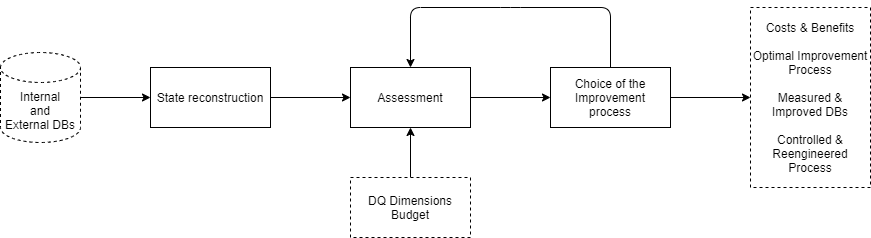
\includegraphics[width=0.9\textwidth]{figures/cdqm-diagram.png}
    \caption{Diagram of the CDQ methodology~\cite{batini2008}}
    \label{fig:cdqm-diagram}
\end{figure}
\FloatBarrier

\subsection{State reconstruction}

TODO

\subsection{Assessment}

TODO

\subsection{Choice of the optimal improvement process}

TODO

\section{BODQ}

Otto et al. (2011) developed a design process for the identification of business oriented DQ metrics~\cite{otto2011}.
The paper does not present any concrete DQ metrics even though they studied data quality problems in three companies.
Instead, those three companies' data problems were used to create an assumption that data defects cause business problems~\cite{otto2011}.
According to Otto et al. (2011), the identification of DQ metrics therefore should be based on how the data impacts process metrics~\cite{otto2011}.

A method engineering (ME) is used to design the framework.
Methodology therefore consists of five components:

\begin{itemize}
    \item design activities,
    \item design results,
    \item meta-model,
    \item roles and
    \item techniques.
\end{itemize}

\subsection{Meta-model}

Otto et al. (2011) describe entities and relations used to characterize the activities of the procedure model~\cite{otto2011}.

\begin{figure}[htb]
    \centering
    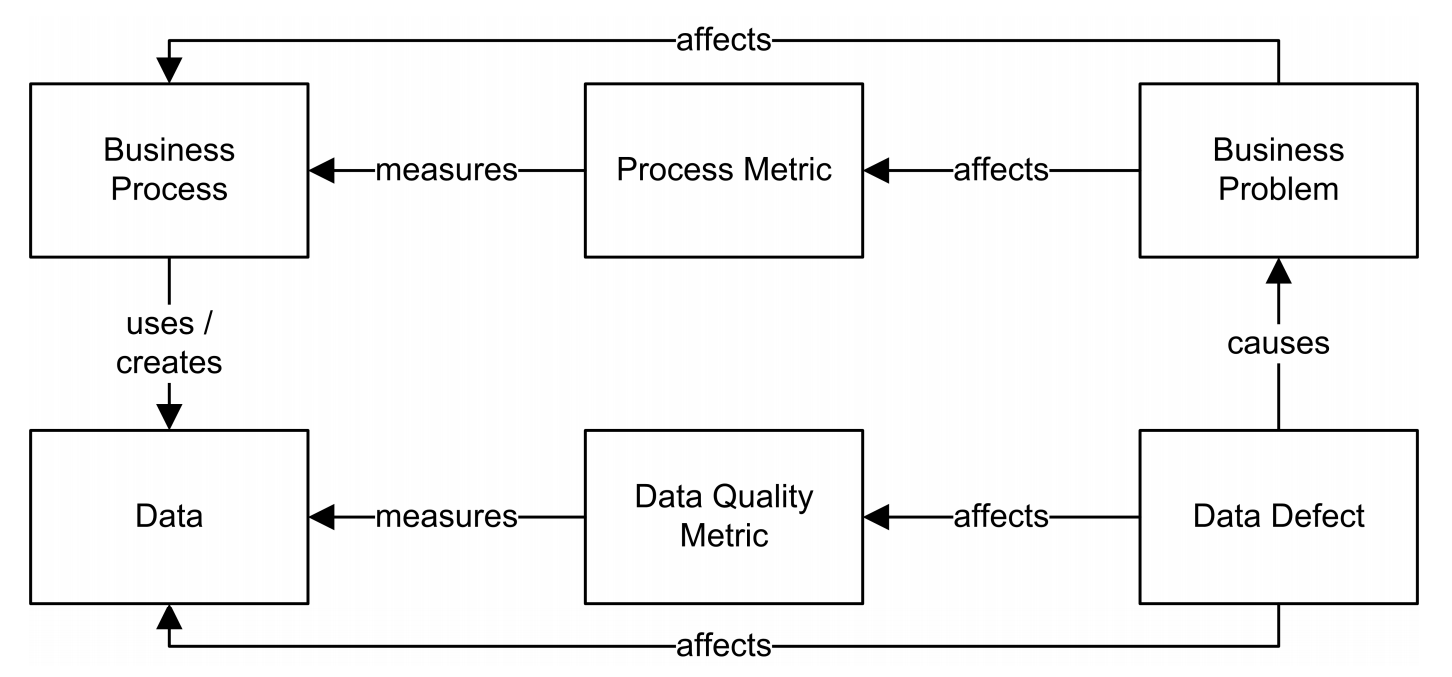
\includegraphics[width=0.9\textwidth]{figures/otto-figure-1.png}
    \caption{Entities and relations of a business oriented data quality metric~\cite{otto2011}}
    \label{fig:otto-figure-1}
\end{figure}
\FloatBarrier

\subsubsection{Business Problem}

Business problem is either system state (e.g. the package cannot be delivered) or incident (e.g. scrap parts production) causing decrease of system performance, therefore impacts \textit{process metrics} results.
It directly impacts business process and is defined by \textit{probability of occurence}\footnotemark and \textit{intensity of impact}\footnotemark.

\footnotetext[1]{Probability of occurence of event \( E \) can be denoted as \( P(E) = \frac{r}{n} \), where \( r \) is number of ways \( E \) can happen from all possible ways \( n \), \( P(E) \in [0, 1] \).}
\footnotetext[2]{
    Intensity of impact is a measure of the time-averaged power density of a wave at a particular location.
    In our case, intesity should be defined as \( I = \frac{\langle BC \rangle}{BA} \), where \( \langle BC \rangle \) is time-averaged business cost of problem and \( BA \) business area through which the problem propagates during certain time frame, \( I \in [0, \inf] \).
    If we define business area as sum of employees impacted by problem and their time spend to solve it, the unit of intensity would be costs per hour.
}

\subsubsection{Business Process}

By business process is meant sequence of tasks intended to generate value for customer and profit for the company.
The business process is controlled and defined as part of a~business strategy with corresponding modeling and measuring tools such as BPMN~2.0 or Key Performance Indicators (KPIs).

\subsubsection{Process Metric}

Quantitative measure of the degree to which a process fulfill a given quality attribute (e.g. scrap rate).

\subsubsection{Data}

Data is representation of objects and object relations.

\subsubsection{Data Defect}

It is an incident (e.g. wrong entered data), causing value decrease of data quality metrics.
As well as \textit{business problem}, a data defect poses a risk in terms of \textit{probability of occurence} and \textit{intensity of impact}.

\subsubsection{Data Quality Metric}

Quantitative measure of the degree to which data fulfill a given quality attribute (e.g. accuracy, consistency, currency,\ldots).

\subsection{Procedure Model}\label{subsec:procedure-model}

Procedure model defined by Otto et al. (2011) consists of three phases and seven activities.
Activity flow model is shown in the figure~\ref{fig:otto-figure-2}.
Letter color codes under the activities indicate degree of usage in the respective companies mentioned in the paper.
Black color means that activity was fully used, grey color means partial usage and white indicates no use at all.

\begin{figure}[htb]
    \centering
    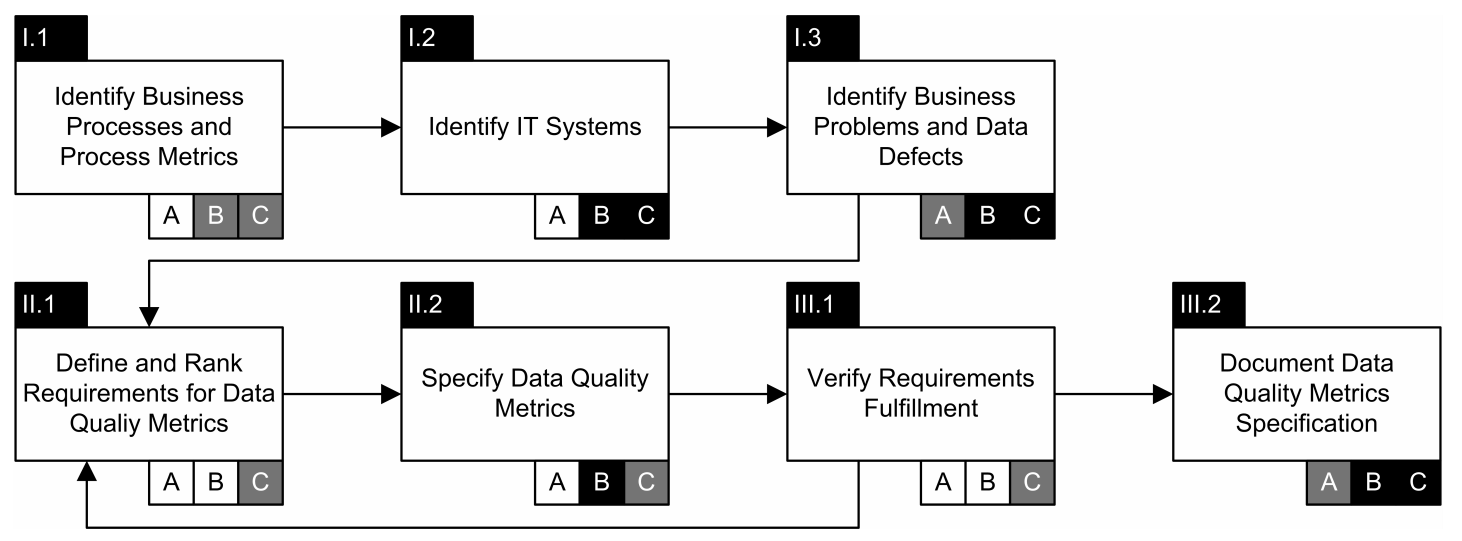
\includegraphics[width=0.9\textwidth]{figures/otto-figure-2.png}
    \caption{Procedure model and degree of usage of activities in each case~\cite{otto2011}}
    \label{fig:otto-figure-2}
\end{figure}
\FloatBarrier

\subsubsection{Phase 1}

First phase is used to collect information.
It consists of three activities:

\begin{enumerate}
    \item Identify Business Processes and Process Metrics,
    \item Identify IT Systems,
    \item Identify Business Problems and Data Defects.
\end{enumerate}

\subsubsection{Phase 2}

Second phase is used to specify requirements and design data quality mestrics.
It consists of two activities:

\begin{enumerate}
    \item Define and Rank Requirements for Data Quality Metrics,
    \item Specify Data Quality Metrics.
\end{enumerate}

\subsubsection{Phase 3}

Third phase is intended to approve and decument results.
As well assecond phase, this one consists of two activities:

\begin{enumerate}
    \item Verify Requirements Fulfillment,
    \item Document Data Quality Metrics Specification.
\end{enumerate}

\subsection{Roles}

In the last part, the authors declare six roles and their assignment to activities from section~\ref{subsec:procedure-model}.
Those roles are:

\begin{itemize}
    \item Chief Data Steward,
    \item Business Data Steward,
    \item Technical Data Steward,
    \item Process Owner,
    \item Process user and
    \item Sponsor.
\end{itemize}

\section{ORME}

Batini et al. (2007) provided DQ assessment methodology called ORME (from italian word \enquote{orme} meaning track or trace).
The methodology consists of four Data Quality Risk evaluation phases:

\begin{enumerate}
    \item prioritization,
    \item identification,
    \item measurement,
    \item monitoring.
\end{enumerate}

In the work, authors provided a comprehensive classification of costs of poor data quality.
In short, they categorized costs into three classes:

\begin{itemize}
    \item current cost of insufficient data quality,
    \item cost of IT/DQ initiative to improve current quality status,
    \item benefits gained from improvement initiative implementation.
\end{itemize}

\subsection{Prioritization}

In this phase the model reconstruction happen.
All the relationships among organization units, processes, services and data are put together and organized e.g. in the form of matrices (database/organization matrix, dataflow/organization matrix, database/process matrix).
The main goal is to provide map of the main data use across data providers, consumers and flows.

\subsection{Identification}

This phase main focus is on identification of loss events and definition of overall economic loss metrics.
In this case, loss can be expressed in 
\begin{enumerate*}[label=(\roman*)]
    \item absolute values (e.g. 100 USD),
    \item a percentage with respect to reference variables (e.g. 10\% of GDP), or
    \item a qualitative evaluation (e.g. low-medium-high).
\end{enumerate*}

\subsection{Measurement}

In this phase actual qualitative and quantitative assessment of data quality is conducted.

\subsection{Monitoring}

The last phase establishes a feedback loop and threshold in the DQ assessment process.
DQ dimensions should be, according to the authors, evaluated periodically.
Therefore quality rule violation allerts and automatic processes should be defined in order to ensure required DQ levels.

Authors suggest discriminant analysis as an easy and effective way of loss event identification.
The goal is to identify loss event based on set of new values in the data source.
The model is build on a training set, with two classes (\textit{loss} and \textit{no loss}) in consideration.
A set of linear functions from predictors is constructed,

\begin{equation*}
    L = b_1 x_1 + b_2 x_2 + \ldots + b_3 x_3 + c
\end{equation*}

where \( b_k \) are discriminant coeficient, \( x_k \) are input variables (predictors) and \( c \) is a constant.

\section{Data Quality Attributes}\label{sec:data-quality-attributes}

Eppler (2006) presented list of seventy of the most used data and information quality criteria explicitly defined in the literature.
They provide criterial basis for most of the DQ frameworks.
The list is shown in the figure~\ref{fig:dq-criteria}.

\begin{figure}[htb]
    \begin{multicols}{3}
        \begin{enumerate}
            \item Comprehensiveness
            \item Accuracy
            \item Clarity
            \item Applicability
            \item Conciseness
            \item Consistency
            \item Correctness
            \item Currency
            \item Convenience
            \item Timeliness
            \item Traceability
            \item Interactivity
            \item Accessibility
            \item Security
            \item Maintainability
            \item Speed
            \item Objectivity
            \item Attributability
            \item Value-added
            \item Reputation (source)
            \item Ease-of-use
            \item Precision
            \item Comprehensibility
            \item Trustworthiness\newline (source)
            \item Reliability
            \item Price 
            \item Verifiability
            \item Testability
            \item Provability
            \item Performance
            \item Ethics
            \item Privacy
            \item Helpfulness
            \item Neutrality
            \item Ease of Manipulation
            \item Validity
            \item Relevance
            \item Coherence
            \item Interpretability
            \item Completeness
            \item Learnability
            \item Exclusivity
            \item Right Amount
            \item Existence of meta information
            \item Appropriateness\newline of meta information
            \item Target group orientation
            \item Reduction of complexity
            \item Response time
            \item Believability
            \item Availability
            \item Consistent Representation
            \item Ability to represent null values
            \item Semantic Consistency
            \item Concise Representation
            \item Obtainability
            \item Stimulating
            \item Attribute granularity
            \item Flexibility
            \item Reflexivity
            \item Robustness
            \item Equivalence of redundant or distributed data
            \item Concurrency of redundant or distributed data
            \item Nonduplication
            \item Essentialness
            \item Rightness
            \item Usability
            \item Cost
            \item Ordering
            \item Browsing
            \item Error rate
        \end{enumerate}
    \end{multicols}

    \centering
    \caption{Data \& Information Quality Criteria~\cite{eppler2006}}
    \label{fig:dq-criteria}
\end{figure}
\FloatBarrier

Two main perspectives on Data Quality Management:

Broad Perspective (from the enterprise poin of view on the lifecycle of data circulating in the company)~\cite{book:dama}
Narrow Perspective (from the viewpoint of tasks to be done by data management professionals)~\cite{pres:dcam}

% \section{Requirements for Data Quality Metrics}

% TODO

% \subsection{Existence of minimum and maximum metric values}

% TODO

% \subsection{Interval-scaled metric values}

% TODO

% \subsection{Quality of the configuration parameters and the determination of the metric values}

% TODO

% \subsection{Sound aggregation of the metric values}

% TODO

% \subsection{Economic efficiency of the metric}

% TODO

% \section{Other}

% \begin{figure}[htb]
%     \centering
%     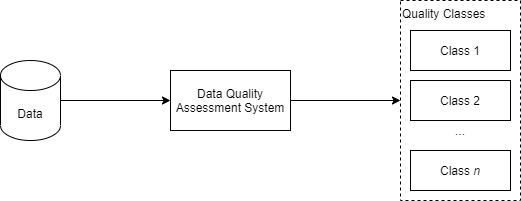
\includegraphics[width=0.9\textwidth]{figures/dq-simple.png}
%     \caption{}
%     \label{fig:dq-simple}
% \end{figure}
% \FloatBarrier

% \begin{figure}[htb]
%     \centering
%     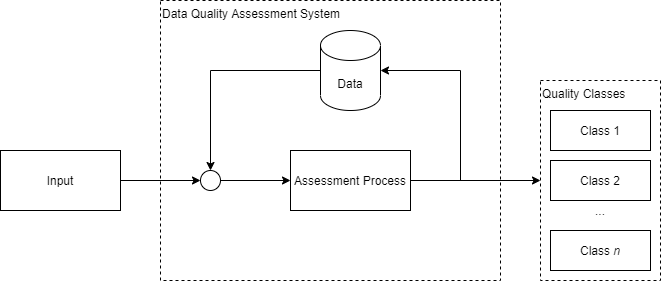
\includegraphics[width=0.9\textwidth]{figures/dq-system.png}
%     \caption{}
%     \label{fig:dq-system}
% \end{figure}
% \FloatBarrier

% \subsection{System Stability}

% In principle, we can classify three types of system stability:

% \begin{enumerate}
%     \item Stable System (Absolute and Conditional stability);
%     \item Marginally Stable System;
%     \item Unstable System.
% \end{enumerate}

% \subsection{Analytics Types}

% \begin{itemize}
%     \item Descriptive – what happened in the past;
%     \item Diagnostic – why something happened in the past;
%     \item Predictive – what is most likely to happen in the future;
%     \item Prescriptive – recommends actions to affect those outcomes.
% \end{itemize}

% DQ dimensions vs DQ metrics

% "Confidetial/secret data will always have limited quality."
